
\documentclass{beamer}
\usetheme{Singapore}
\usecolortheme[RGB={0,32,91}]{structure}  % Rice blue
\setbeamertemplate{navigation symbols}{\insertframenumber}

\title{A survey-lite of tracking-based soccer research}
\author{SMGT 432}

\begin{document}

  \begin{frame}
    \maketitle
  \end{frame}

  \begin{frame}{Outline}
    \footnotesize
    \begin{columns}
      \begin{column}{0.5\textwidth}
        2016:
        \begin{itemize}
          \item Spearman (Opta)
        \end{itemize}
        2017:
        \begin{itemize}
          \item Spearman (Sloan)
          \item Power {\it et al.} (KDD)
        \end{itemize}
        2018:
        \begin{itemize}
          \item Spearman (Sloan)
          \item Fernandez and Bornn (Sloan)
        \end{itemize}
      \end{column}
      \begin{column}{0.5\textwidth}
        2019:
        \begin{itemize}
          \item Fernandez {\it et al.} (Sloan)
          \item Shaw and Glickman (Barcelona)
        \end{itemize}
        2021:
        \begin{itemize}
          \item Shaw and Gopaladesikan (Sloan)
        \end{itemize}
        2022:
        \begin{itemize}
          \item Everett {\it et al.} (StatsBomb)
        \end{itemize}
      \end{column}
    \end{columns}
  \end{frame}

  \begin{frame}{Spearman (2016 Opta Forum)}{Quantifying Pitch Control}
    \centering
    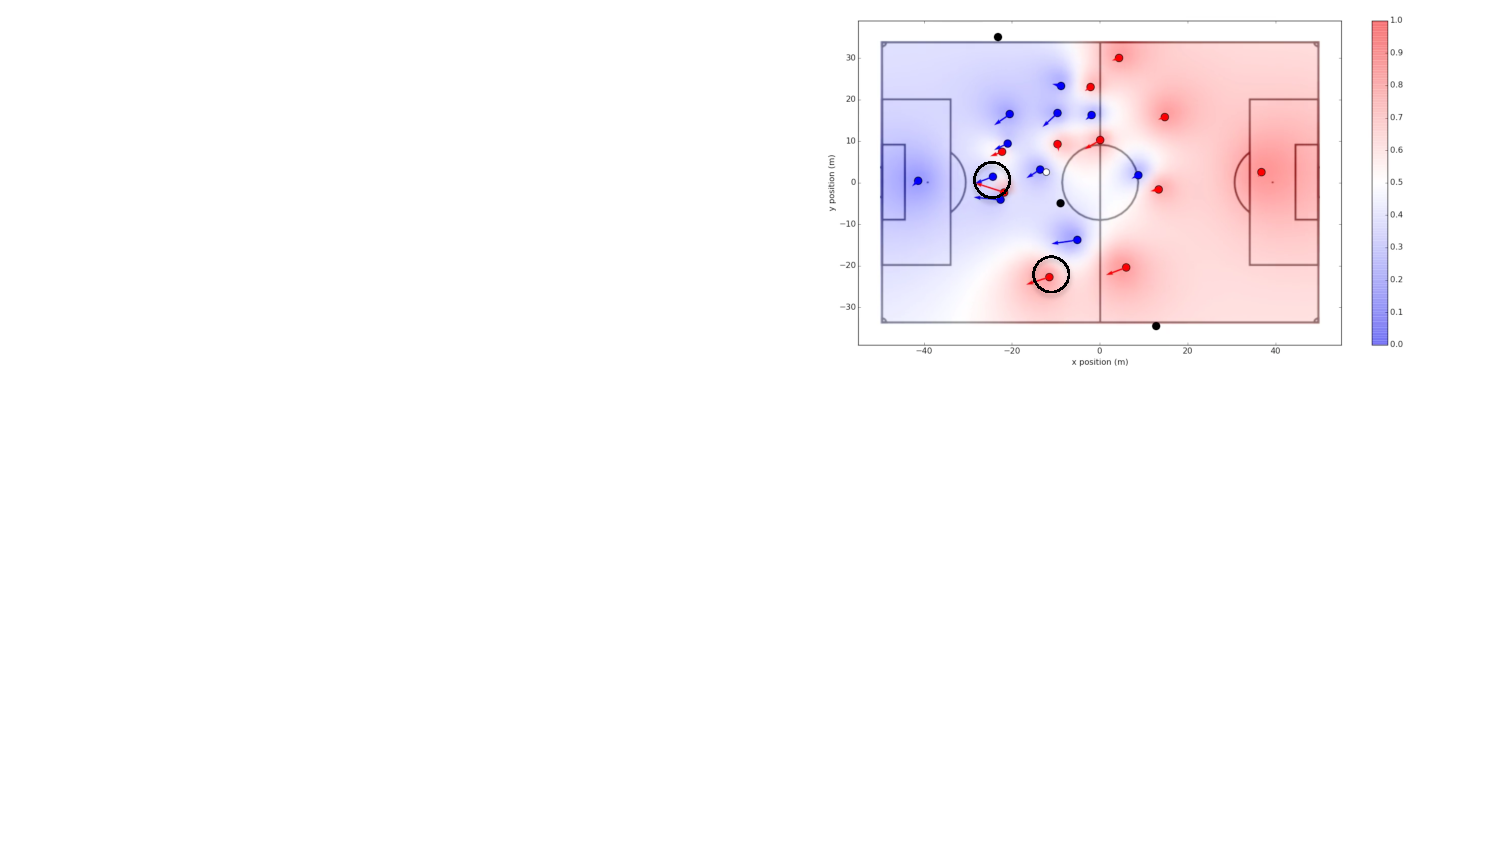
\includegraphics[width=0.8\textwidth]{images/spearman_2016.pdf}
    $$
      PCF(t_i, \ell_i) = \left[\frac{\sum_i \ell_it_i^\beta}{\sum_i t_i^\beta} + 1\right] / 2
    $$
  \end{frame}

  \begin{frame}{Spearman (2016 Opta Forum)}{Quantifying Pitch Control}
    Data:
      \begin{itemize}
        \item TRACAB (provided by the forum)
      \end{itemize}
    Calculating times using:
    \begin{itemize}
      \item Player position
      \item Player velocity
      \item Player acceleration
      \item Maximum player speed
    \end{itemize}
    Applications:
    \begin{itemize}
      \item A new way to watch film
      \item A new metric for player performance
      \item Player positioning
    \end{itemize}
    Citations: 7
  \end{frame}

  \begin{frame}{Spearman {\it et al.} (2017 Sloan Conference)}{Physics-Based Modeling of Pass Probabilities in Soccer}
    \centering
    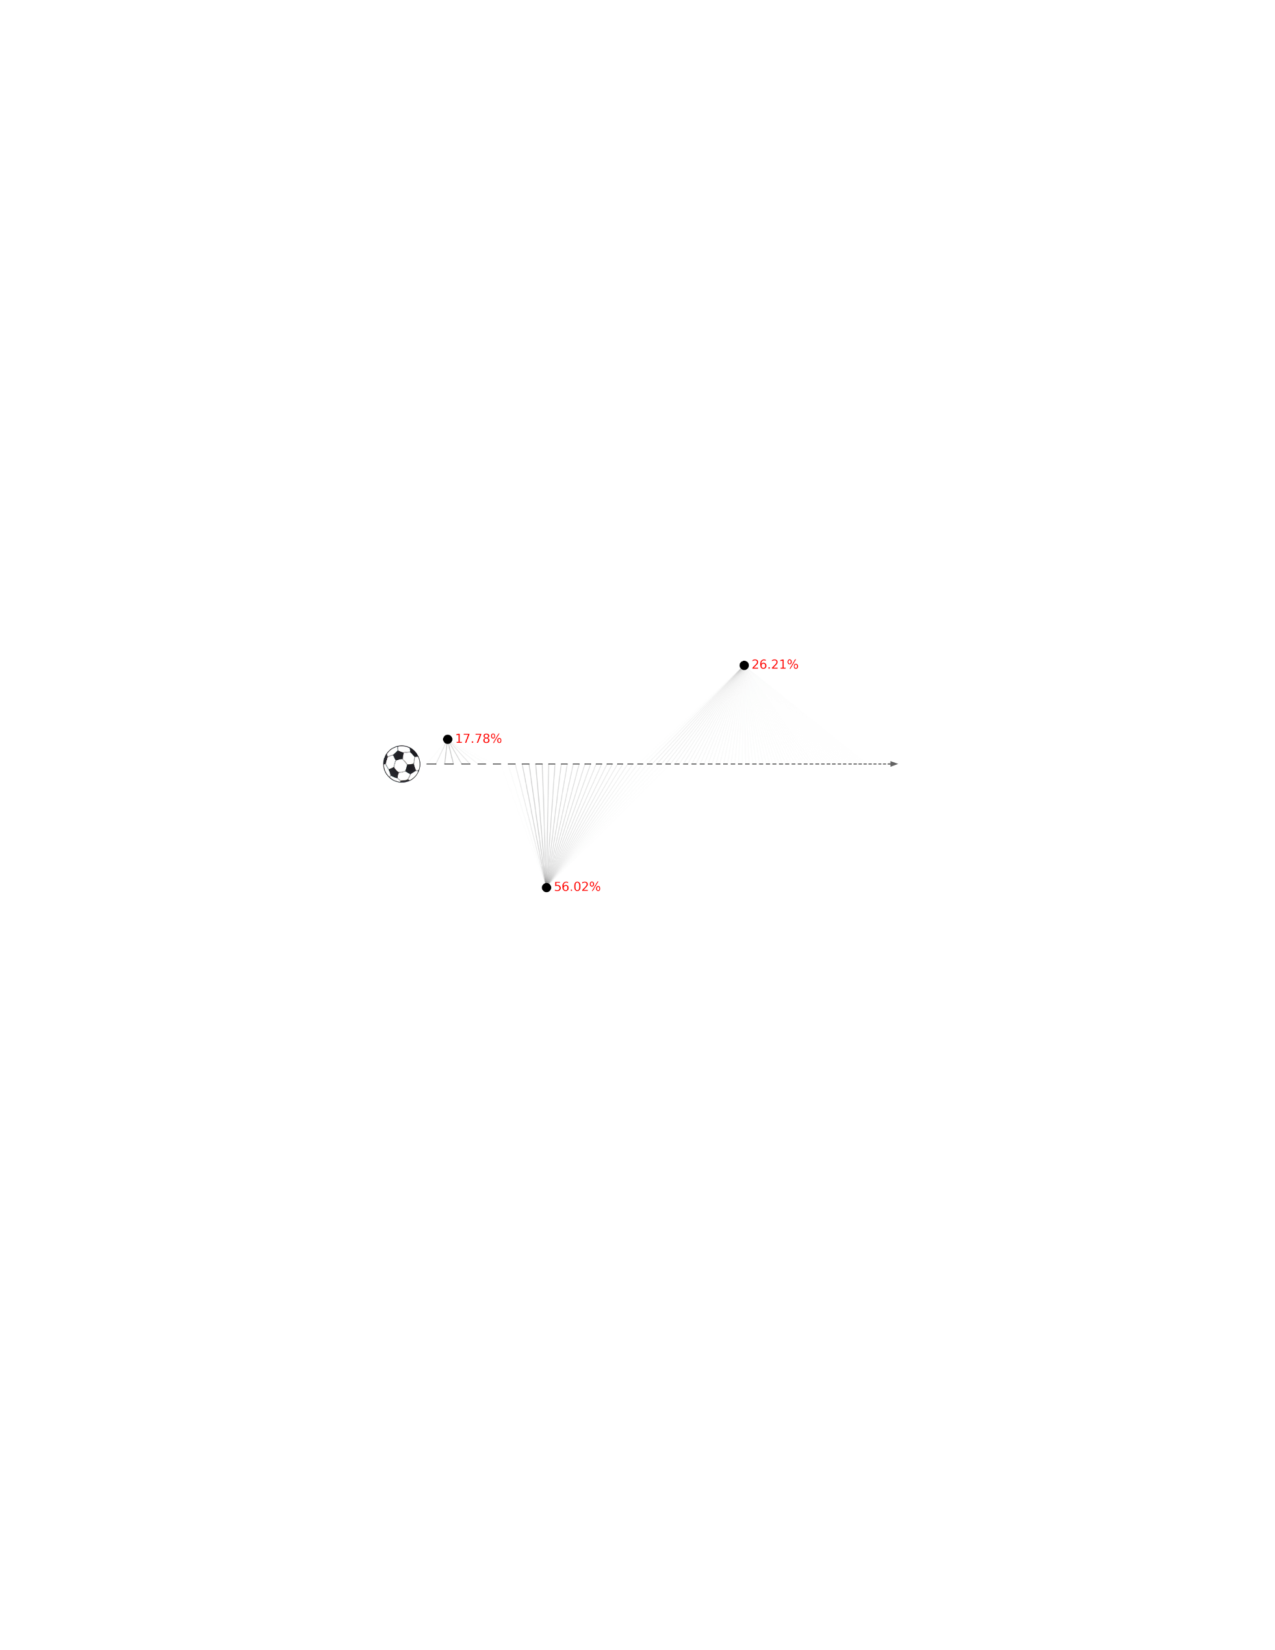
\includegraphics[width = 0.8\textwidth]{images/spearman_etal_2017.pdf}
  \end{frame}

  \begin{frame}{Spearman {\it et al.} (2017 Sloan Conference)}{Physics-Based Modeling of Pass Probabilities in Soccer}
    Data:
    \begin{itemize}
      \item 38 matches from 2015-16 EPL (provided by Crystal Palace)
    \end{itemize}
    Applications:
    \begin{itemize}
      \item Pitch control
      \item Hypothetical passing
    \end{itemize}
    Citations: 101
  \end{frame}

  \begin{frame}{Power {\it et al.} (2017 KDD Workshop)}
    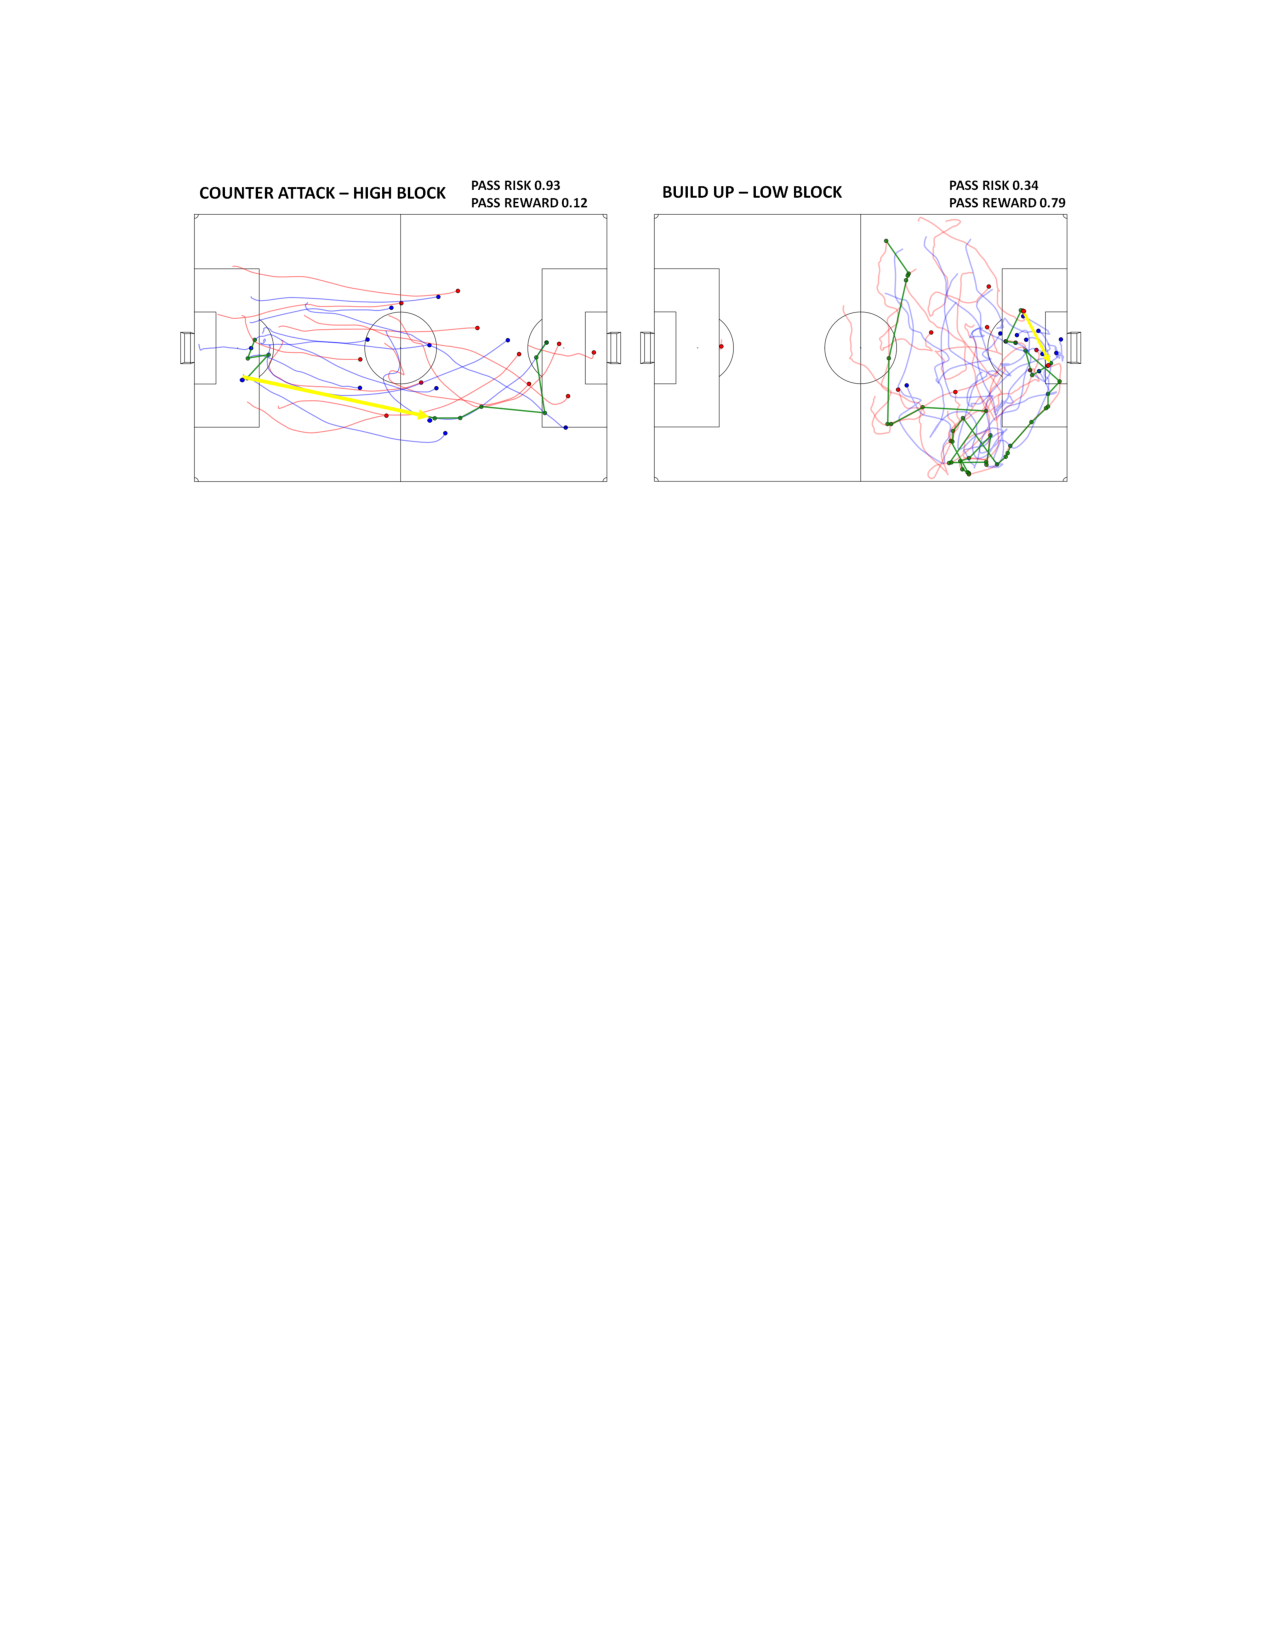
\includegraphics[width = \textwidth]{images/power_etal_2017.pdf}
  \end{frame}


  \begin{frame}{Power {\it et al.} (2017 KDD Workshop)}
    \small
    Data:
    \begin{itemize}
      \item 726 matches from 2014-2016 EPL (provided by STATS)
    \end{itemize}
    Features:
    \begin{itemize}
      \item Speed of the player in possession and the intended receiver
      \item Speed of the nearest defender toward the passer and the receiver
      \item Distance of nearest defender to the passer and receiver
      \item Nearest defender angle to the passing line
      \item First time pass
      \item Time from regaining possession
    \end{itemize}
    Applications:
    \begin{itemize}
      \item Match analysis
      \item Ranking the riskiest players
      \item Ranking of best players receiving passes
    \end{itemize}
    Citations: 133
  \end{frame}

  \begin{frame}{Spearman (2018 Sloan Conference)}{Beyond Expected Goals}
    \centering
    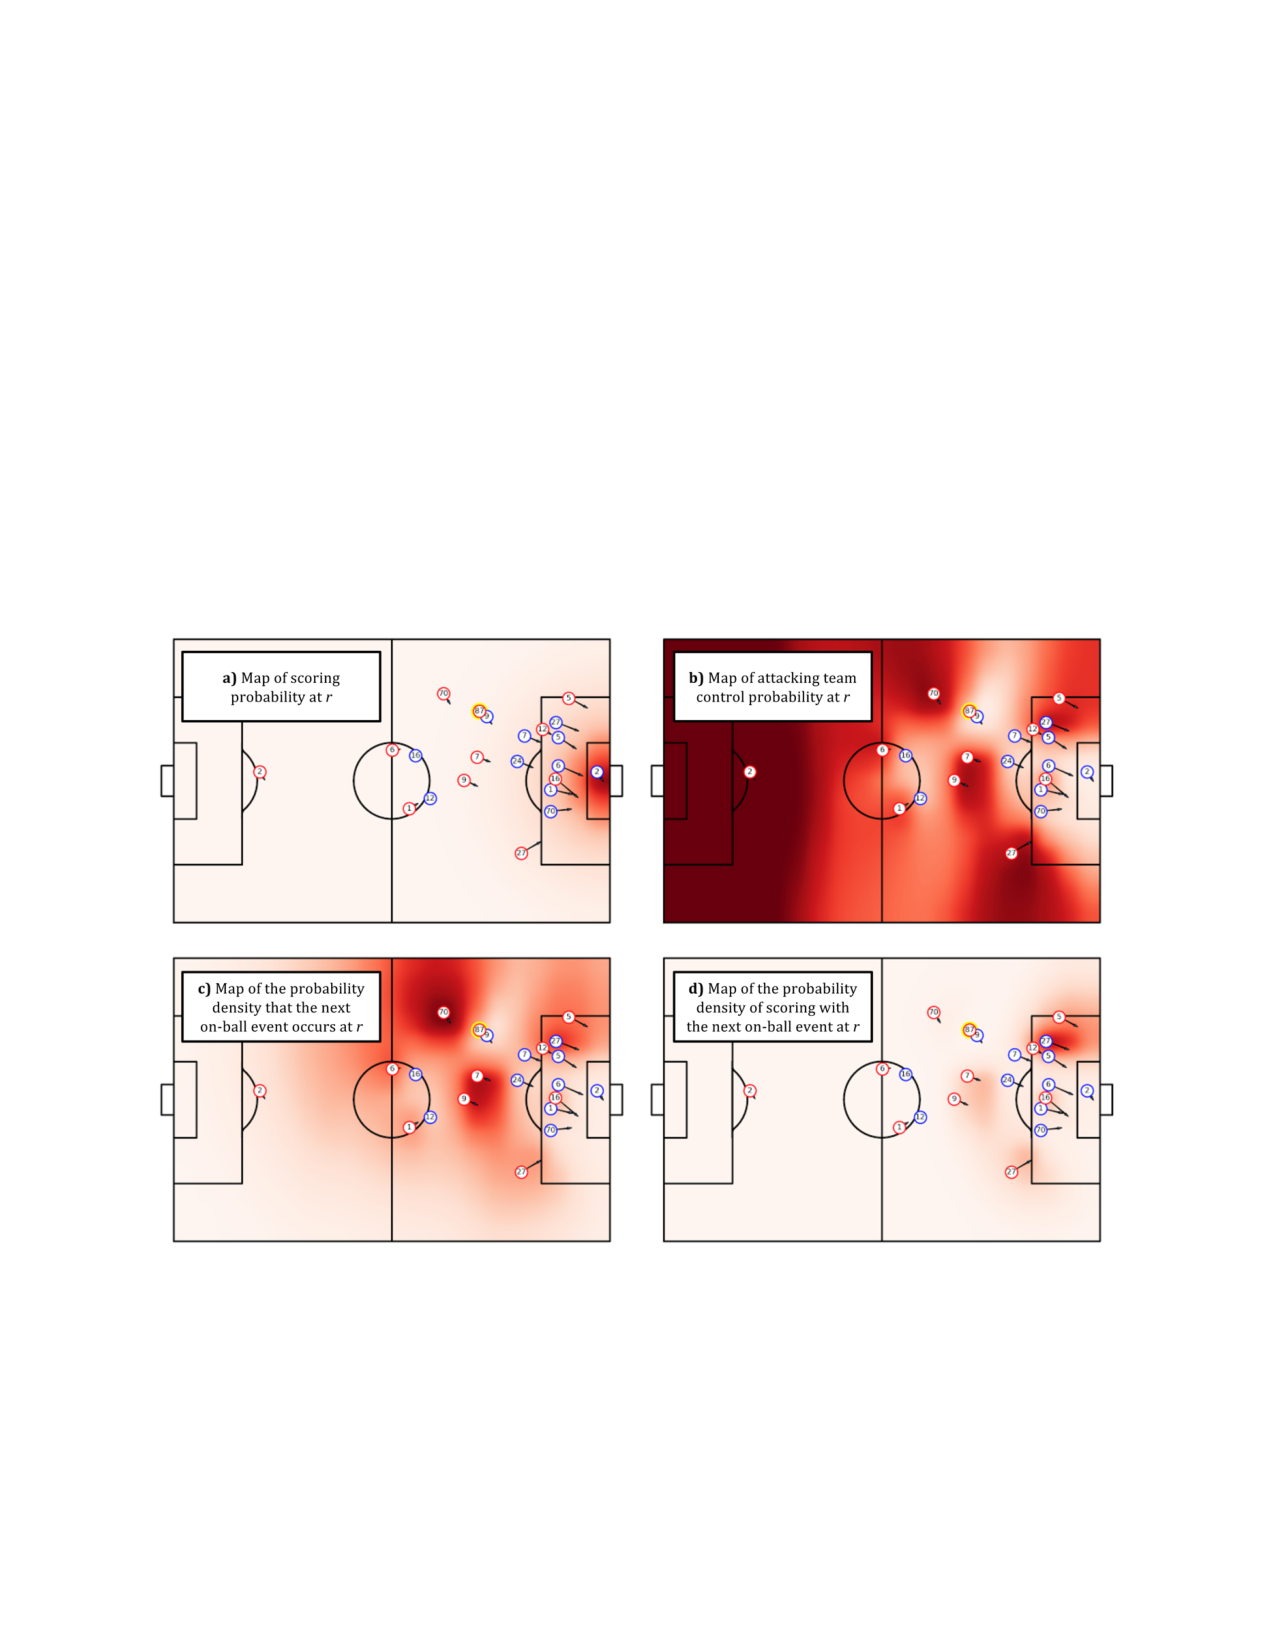
\includegraphics[width = 0.8\textwidth]{images/spearman_2018.pdf}
    $$
      P(G | D) = \sum_{r \in \mathbb{R}\times\mathbb{R}} P(S_r | C_r, T_r, D) P(C_r | T_r, D) P(T_r | D)
    $$
  \end{frame}

  \begin{frame}{Spearman (2018 Sloan Conference)}{Beyond Expected Goals}
    Data:
    \begin{itemize}
      \item 58 matches of tracking from 2017-2018 (provided by Hudl)
    \end{itemize}
    Applications:
    \begin{itemize}
      \item Tactical moment analysis
      \item Match analysis
      \item Team performance
      \item Player performance
    \end{itemize}
    Citations: 133
  \end{frame}

  \begin{frame}{Fernandez and Bornn (2018 Sloan Conference)}{Wide Open Spaces:\\ A statistical technique for measuring space creation in professional soccer}
    \centering
    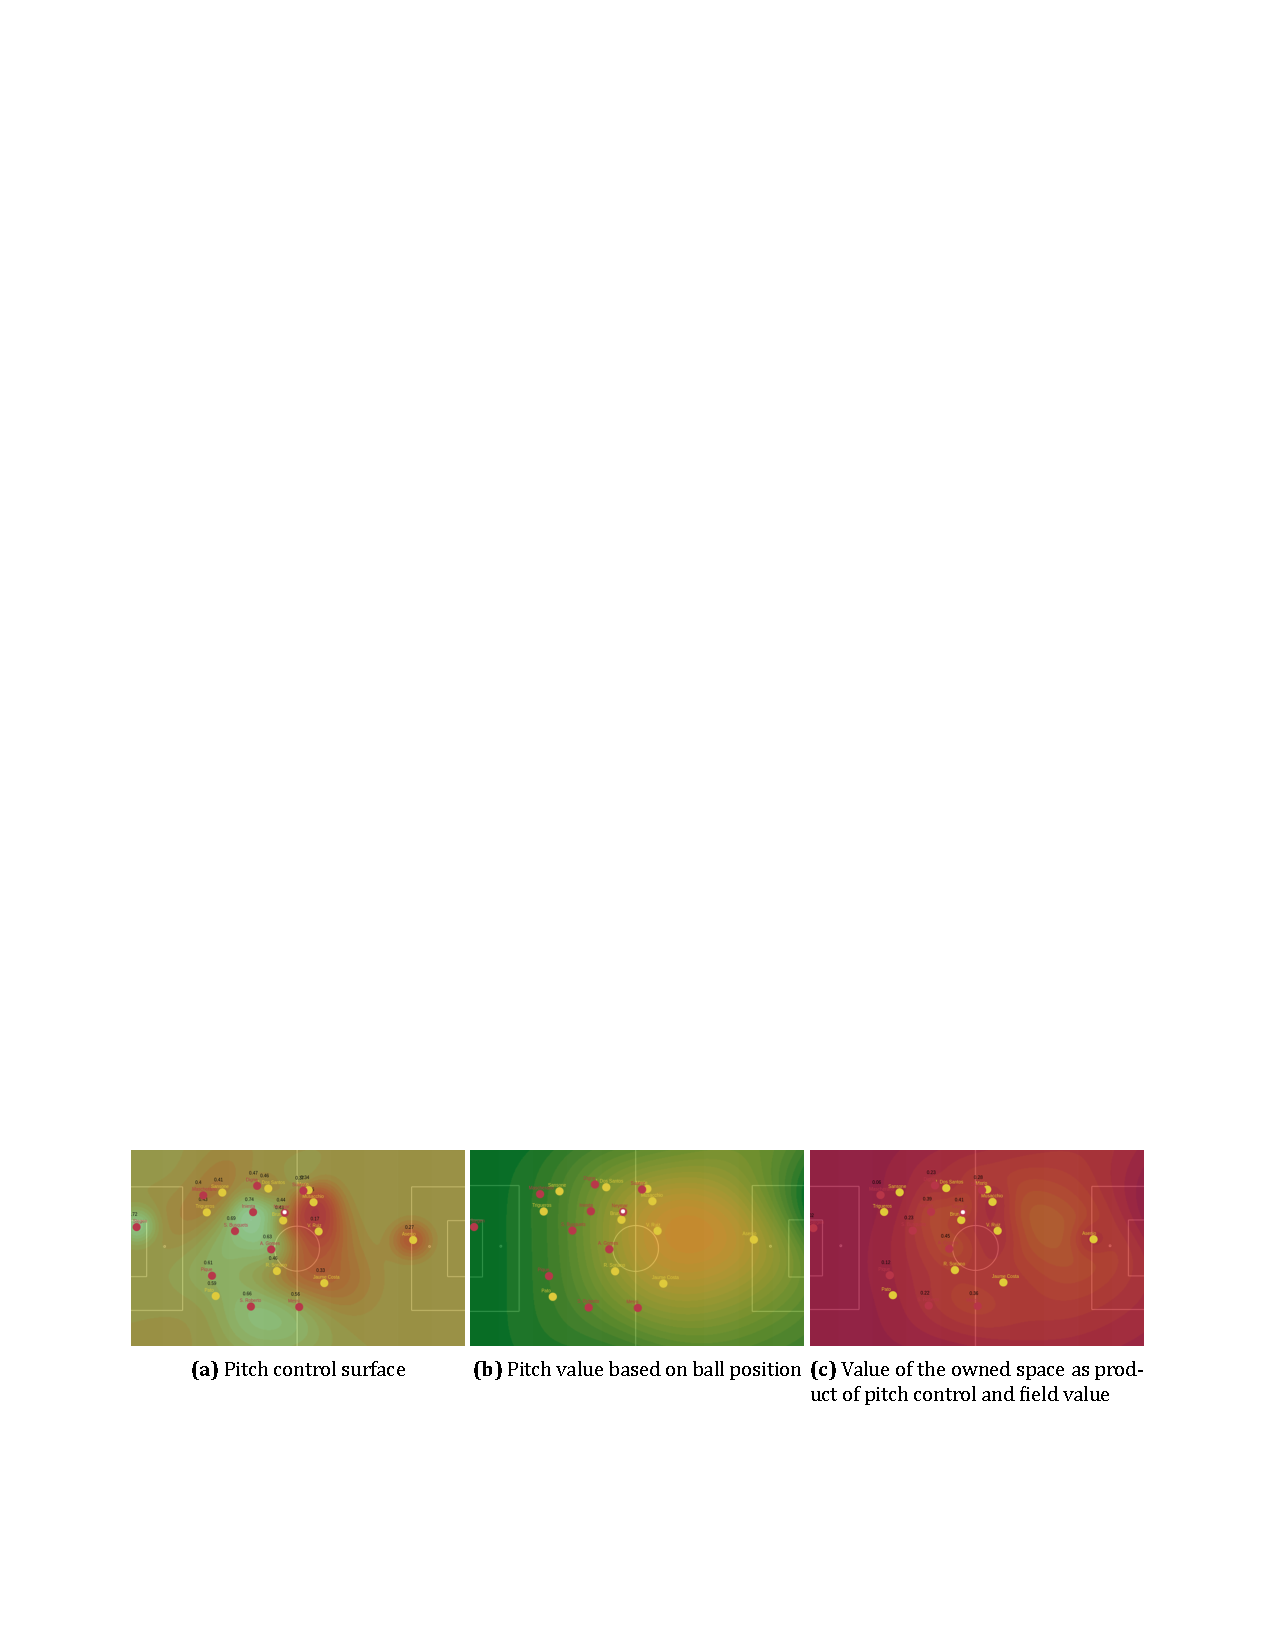
\includegraphics[width = \textwidth]{images/fernandez_bornn_2018.pdf}\\
    $$Q_i(t) = PC_i(t)V(t)$$
  \end{frame}

  \begin{frame}{Fernandez and Bornn (2018 Sloan Conference)}{Wide Open Spaces:\\ A statistical technique for measuring space creation in professional soccer}
    Data:
    \begin{itemize}
      \item 20 matches of Metrica from Spain (provided by Barcelona)
    \end{itemize}
    Citations: 170
  \end{frame}

  \begin{frame}{Fernandez {\it et al.} (2019 Sloan Conference)}{Decomposing the immeasurable sport:\\ A deep learning expected possession value framework for soccer}
    \centering
    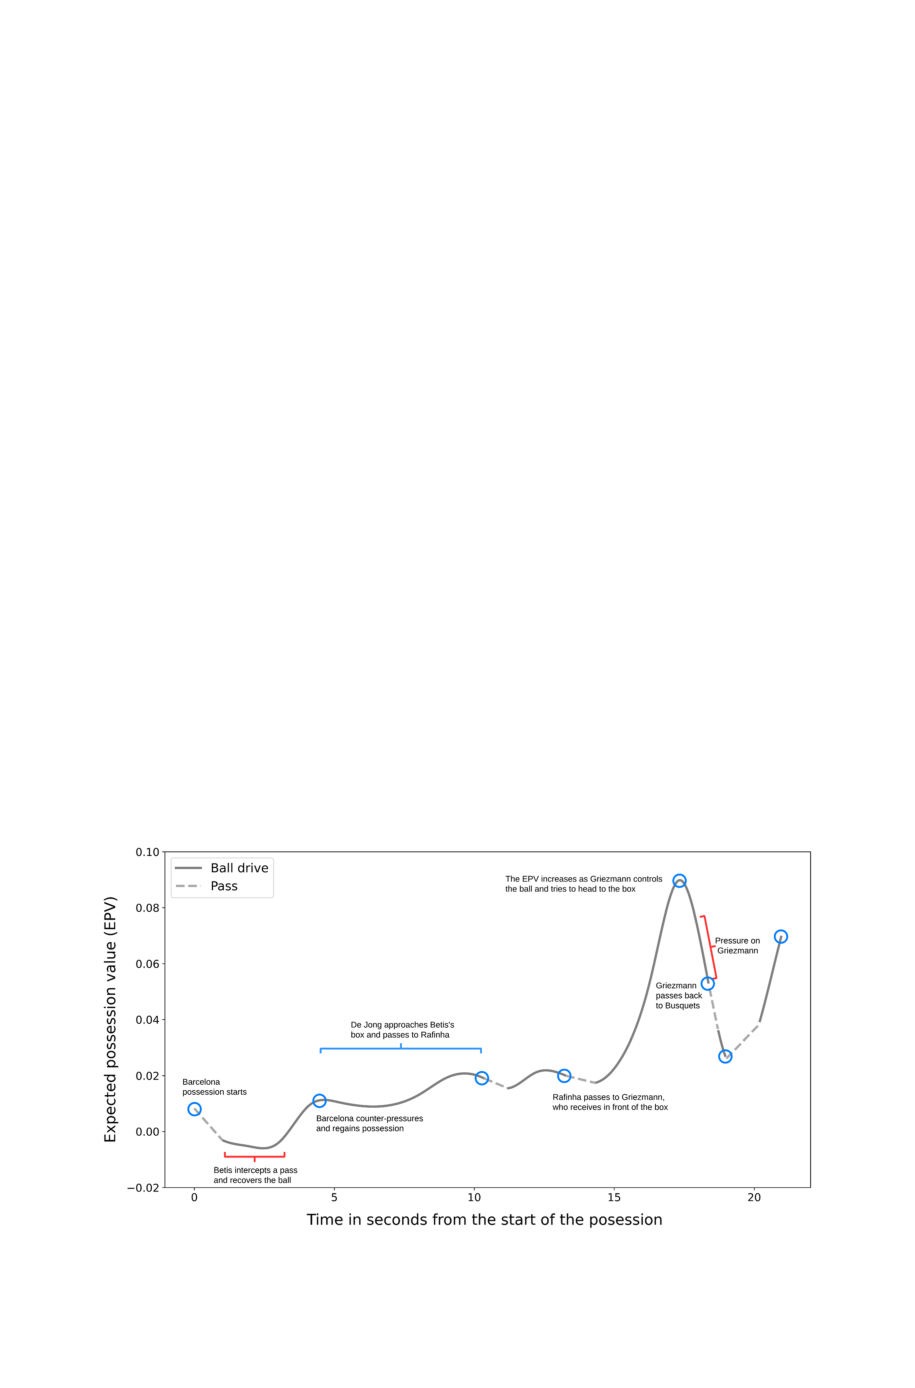
\includegraphics[width = 0.8\textwidth]{images/fernandez_etal_2021.pdf}
    \small
    $$
      EPV(t) = E[X | A = \rho] P(A = \rho) + E[X | A = \varsigma] P(A = \varsigma) + E[X | A = \delta] P(A = \delta)
    $$
  \end{frame}

  \begin{frame}{Fernandez {\it et al.} (2019 Sloan Conference)}{Decomposing the immeasurable sport:\\ A deep learning expected possession value framework for soccer}
    Data:
    \begin{itemize}
      \item Tracking data from 2012-13 EPL (provided by STATS)
      \item Footovision from 2017-18 and 2018-19 FC Barcelona matches (provided by FC Barcelona)
    \end{itemize}
    Applications:
    \begin{itemize}
      \item Pass analysis
      \item Distilling off-ball value creation
      \item Decision-making analysis
    \end{itemize}
    Citations: 148
  \end{frame}

  \begin{frame}{Shaw and Glickman (2019 Barcelona Summit)}{Dynamic analysis of team strategy in professional football}
    \centering
    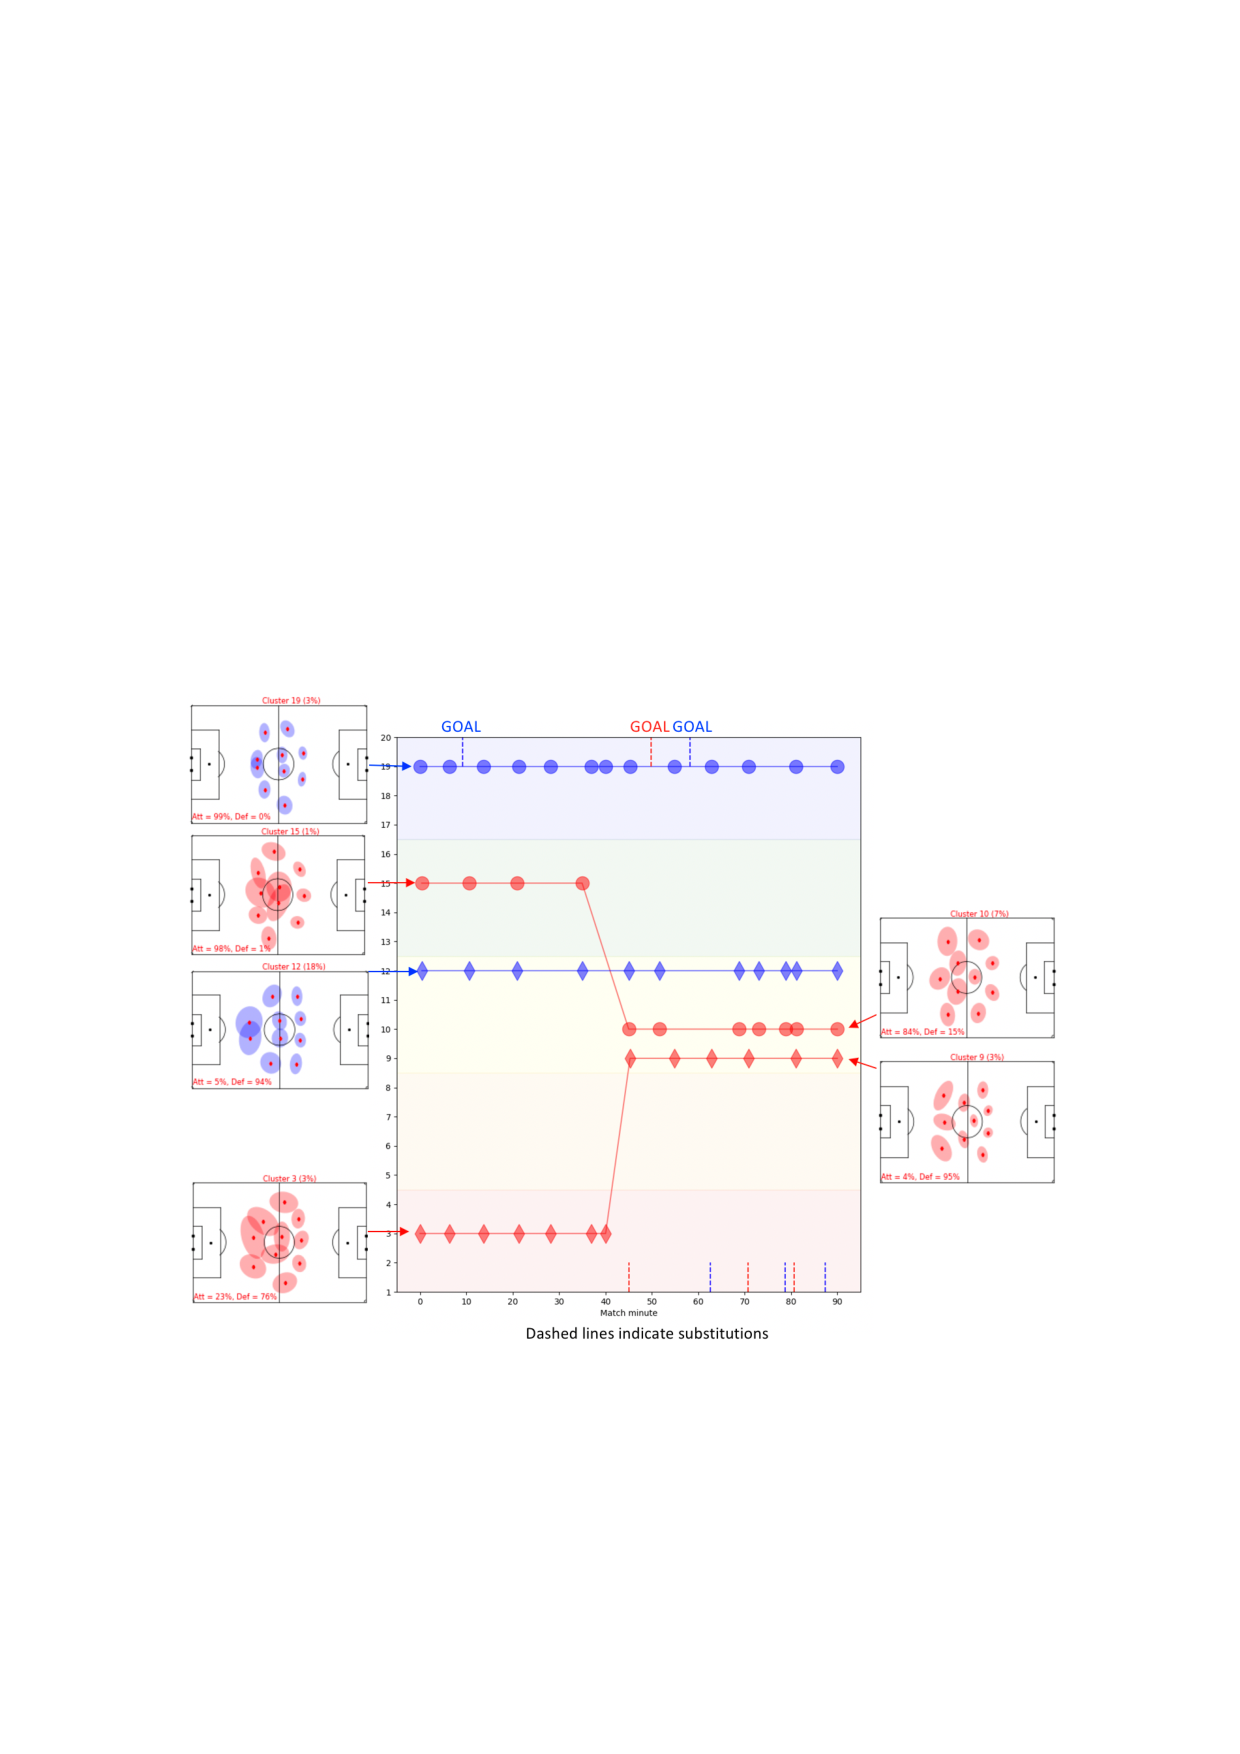
\includegraphics[width = 0.8\textwidth]{images/shaw_glickman_2019.pdf}
  \end{frame}

  \begin{frame}{Shaw and Glickman (2019 Barcelona Summit)}{Dynamic analysis of team strategy in professional football}
    Data:
    \begin{itemize}
      \item 180 matches from ``an elite professional league''
    \end{itemize}
    Applications:
    \begin{itemize}
      \item Exploit opposition tactical changes
      \item Identify weaknesses of specific formations
      \item Consider formation in specific phases of possession
    \end{itemize}
    Citations: 37
  \end{frame}

  \begin{frame}{Shaw and Gopaladesikan (2021 Sloan Conference)}{Routine Inspection: A playbook for corner kicks}
    \centering
    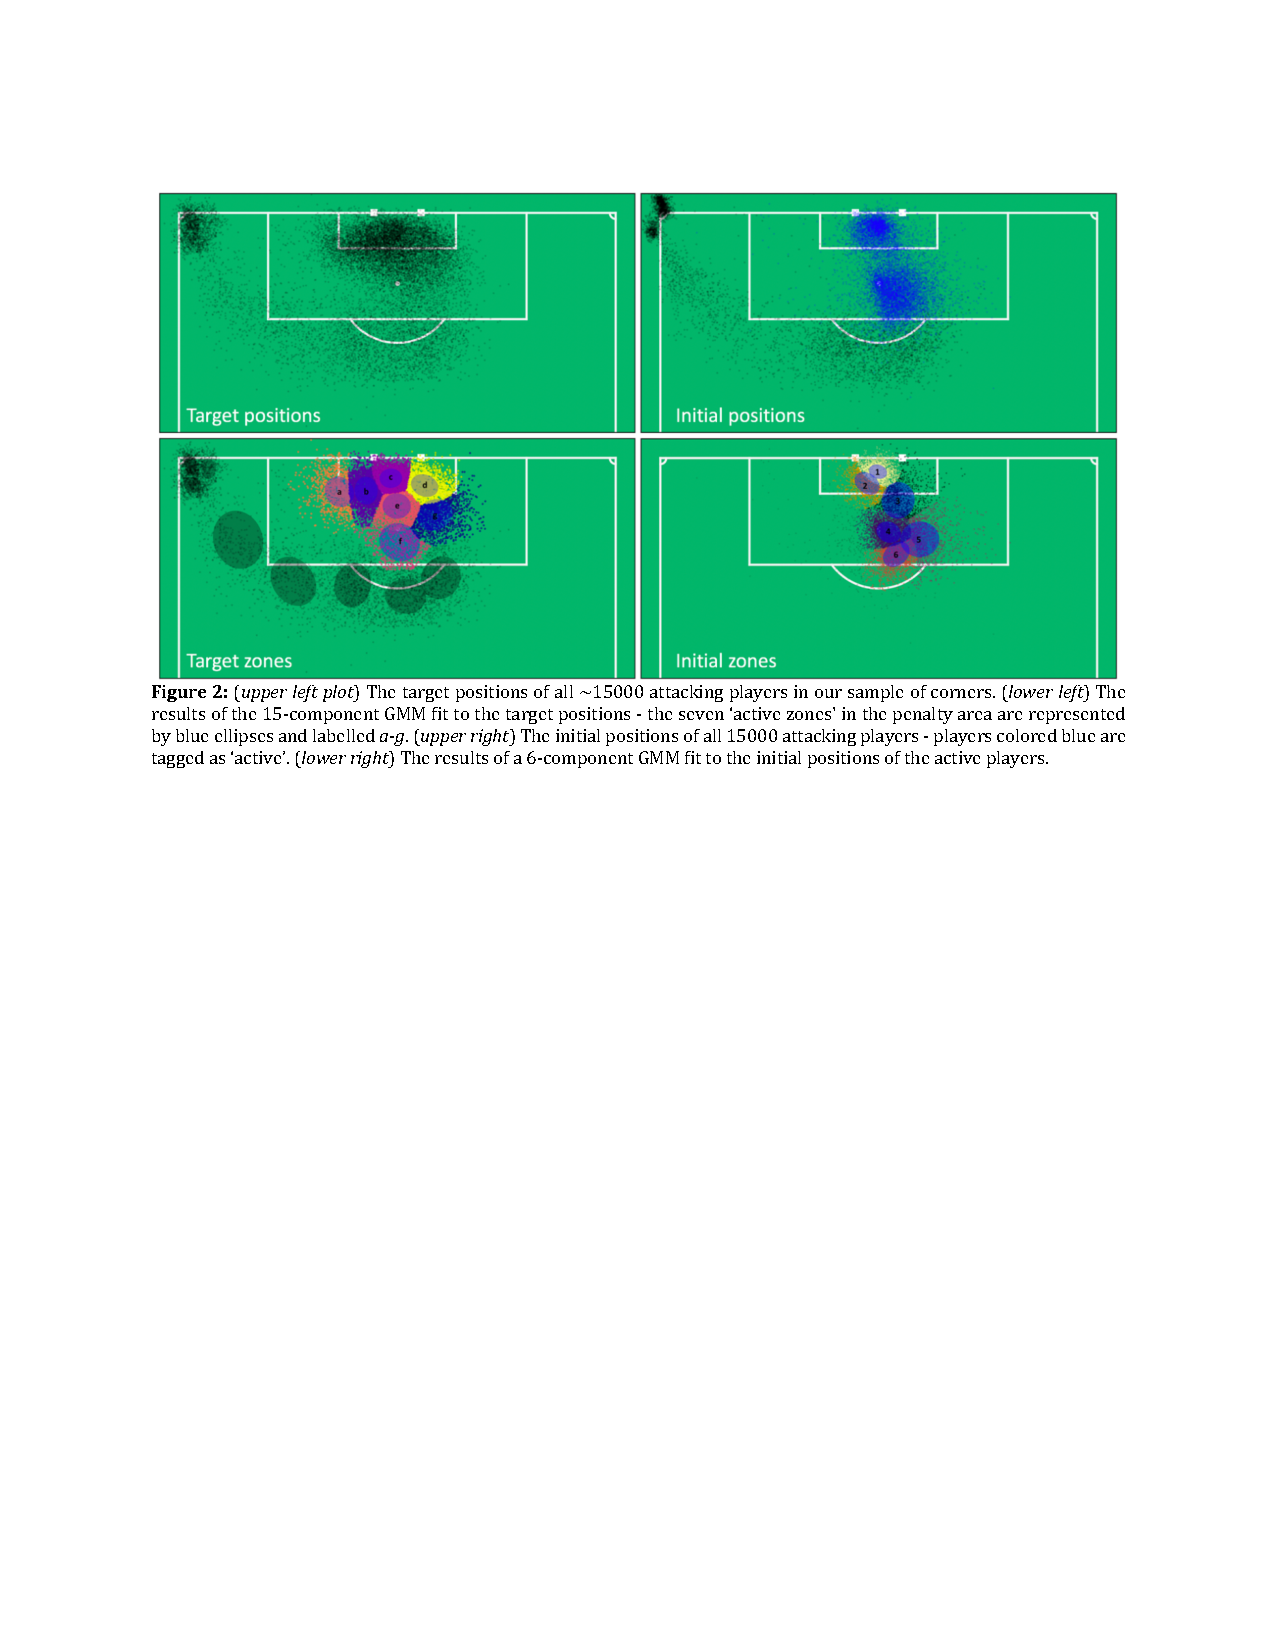
\includegraphics[width = \textwidth]{images/shaw_gopaladesikan_2021.pdf}
  \end{frame}

  \begin{frame}{Shaw and Gopaladesikan (2021 Sloan Conference)}{Routine Inspection: A playbook for corner kicks}
    Data:
    \begin{itemize}
      \item 234 matches from ``an elite European professional league'' (presumably provided by SL Benfica)
    \end{itemize}
    Methods:
    \begin{itemize}
      \item Gaussian mixture modeling
      \item Non-negative matrix factorization
      \item Gradient boosting (for defensive role classification)
    \end{itemize}
    Applications:
    \begin{itemize}
      \item Analysis of an opponent's offensive corner strategies
      \item Comparing the effectiveness of zonal systems
      \item Training optimization
    \end{itemize}
    Citations: 12
  \end{frame}

  \begin{frame}{Everett {\it et al.} (2022)}{Contextual Expected Threat using Spatial Event Data}
    \centering
    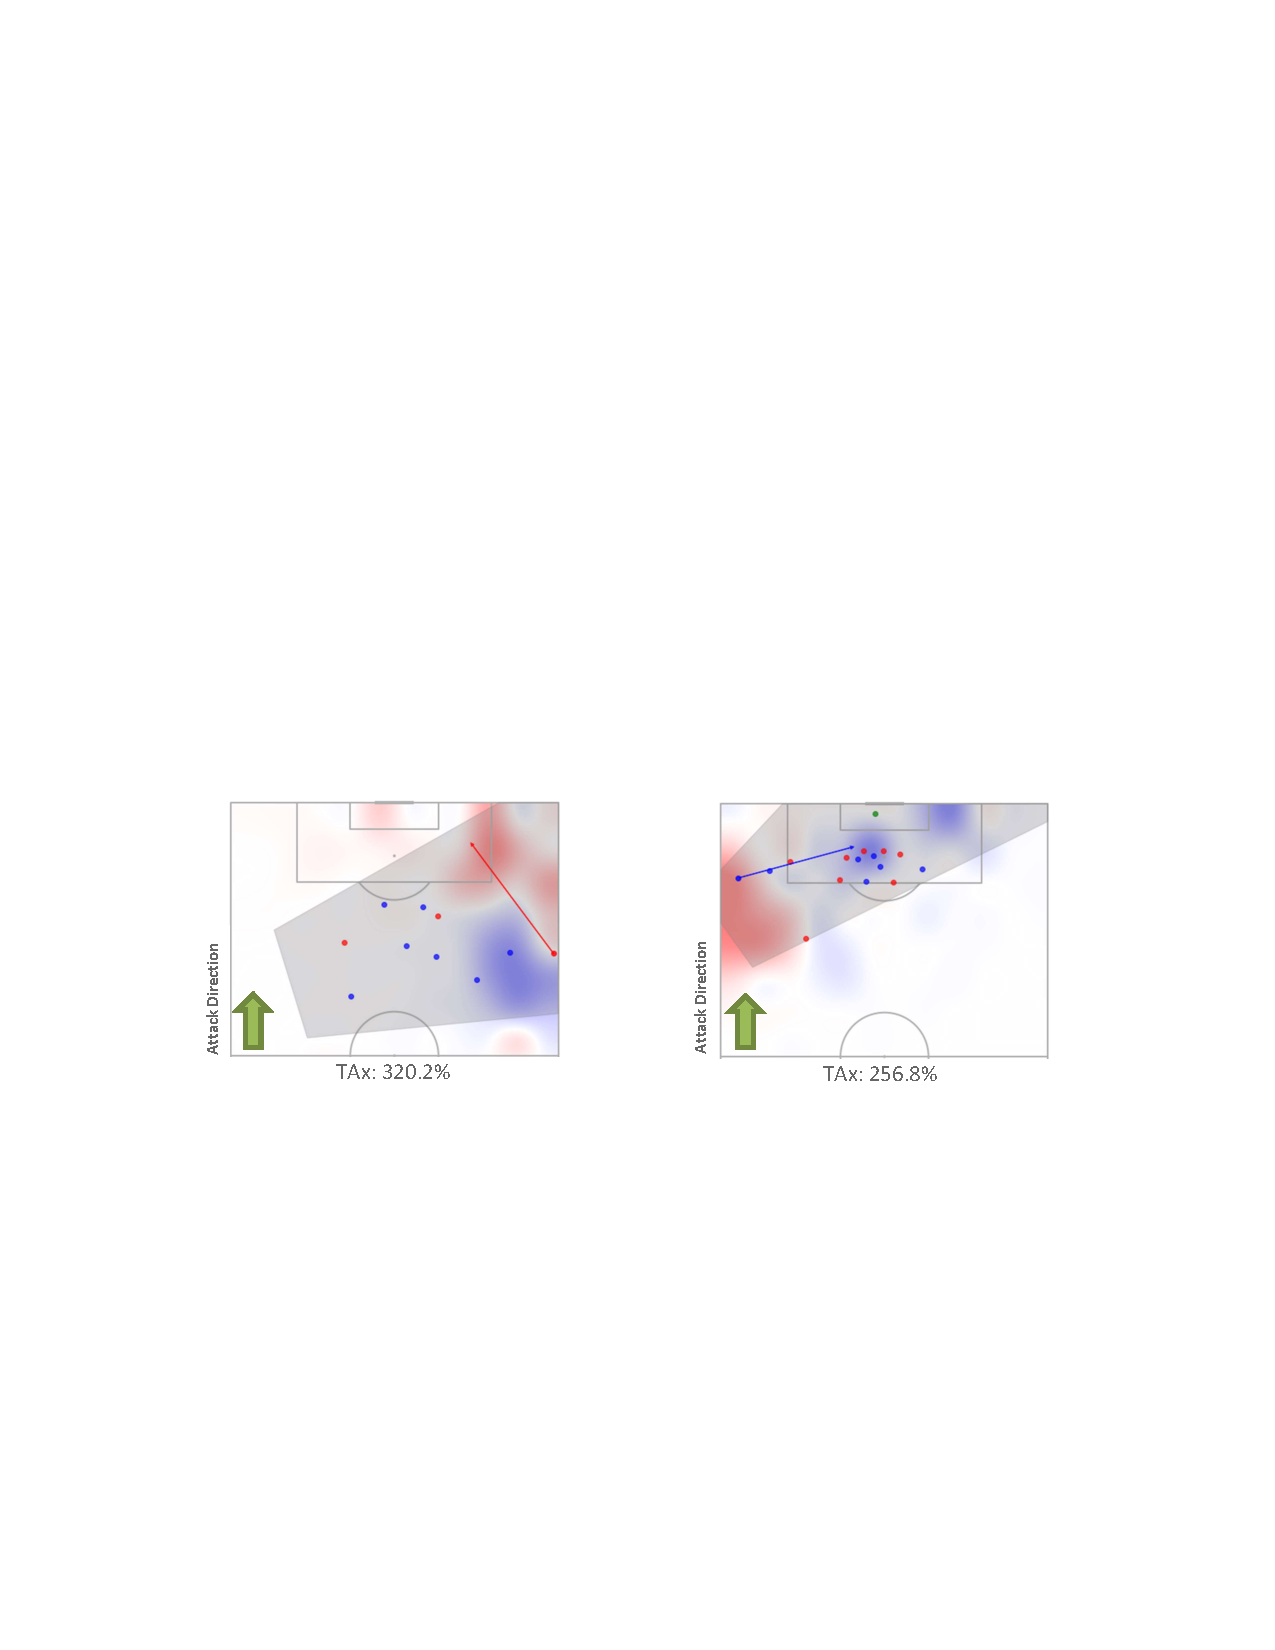
\includegraphics[width = 0.7\textwidth]{images/everett_etall_2022_hi.pdf}\\
    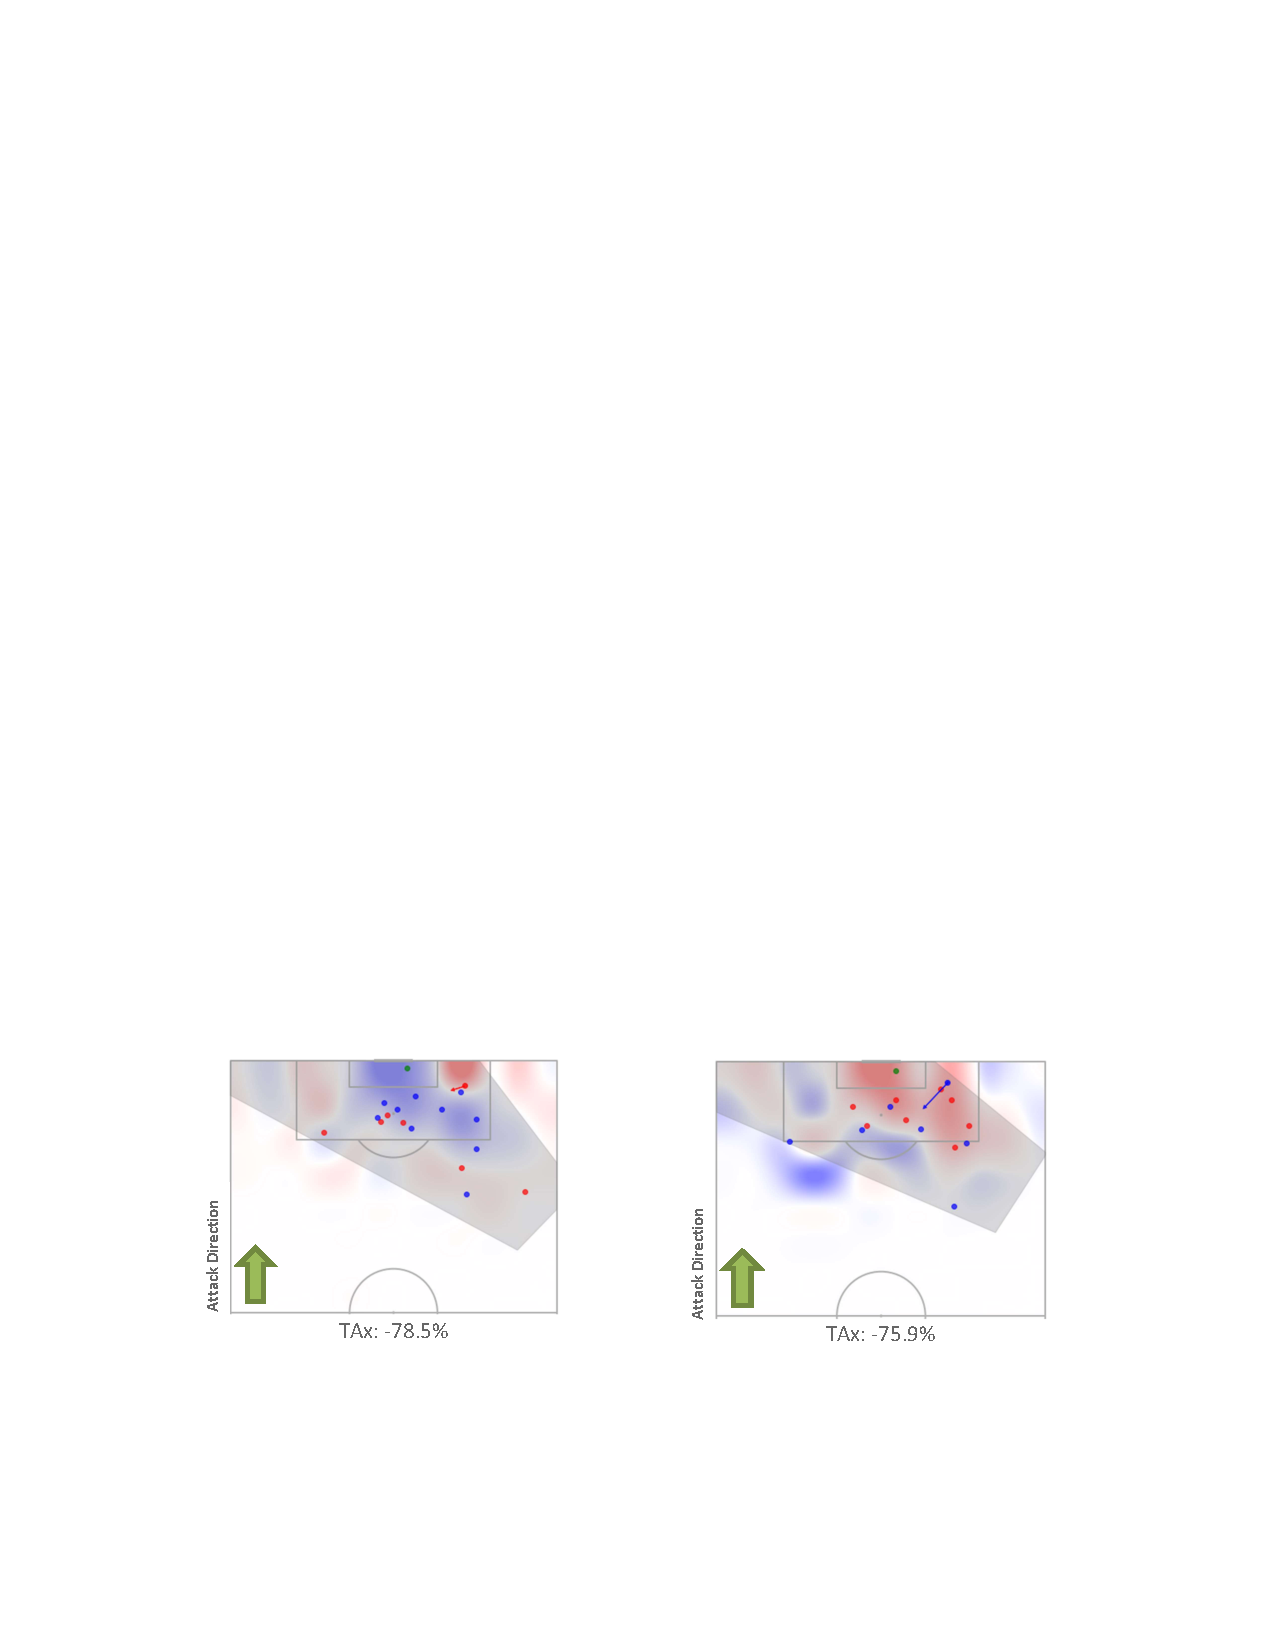
\includegraphics[width = 0.7\textwidth]{images/everett_etall_2022_lo.pdf}
    $$\mbox{TAx} = 100 \times \frac{\mbox{xT}_{spatial} - \mbox{xT}_{original}}{\mbox{xT}_{original}}$$
  \end{frame}

  \begin{frame}{Everett {\it et al.} (2022)}{Contextual Expected Threat using Spatial Event Data}
    Data:
    \begin{itemize}
      \item SB360 data from 2021-22 EPL (provided by StatsBomb)
    \end{itemize}
    Methods:
    \begin{itemize}
      \item Convolutional neural network
    \end{itemize}
    Applications:
    \begin{itemize}
      \item More accurate possession value model
      \item Thread Above Expected
      \item Defensive Optimizer
    \end{itemize}
    Citations: 1
  \end{frame}

\end{document}